
\begin{frame}{}

    \begin{columns}
        \column{.48\textwidth}
        \begin{figure}[H]
            \centering
            \includegraphics[scale = 0.7]{ch2/ntpr.pdf}

        \end{figure}
        \column{.48\textwidth}
        % Różne topologie pseudo-rezystorów z niekontrolowaną wartością rezystancji zaimplementowane w przedwzmacniaczu ze sprzężeniem zmiennoprądowym.        
 
    \end{columns}


\end{frame}

\begin{frame}{}

    \begin{columns}
        \column{.48\textwidth}
        \begin{figure}[H]
            \centering
            \includegraphics[scale = 0.7]{ch2/tpr.pdf}

        \end{figure}
        \column{.48\textwidth}
        % Różne topologie pseudo-rezystorów z kontrolowaną wartością rezystancji zaimplementowane w przedwzmacniaczu ze sprzężeniem zmiennoprądowym.

    \end{columns}


\end{frame}




\begin{frame}{}
    \begin{columns}
        \column{.48\textwidth}
        \begin{figure}[H]
            \centering
            \includegraphics[scale = 0.7]{ch3/fig1-ac_standard.pdf}
        \end{figure}

        \column{.48\textwidth}
        \begin{figure}[H]
            \centering
            \includegraphics[scale = 0.7]{ch3/fig1-ac_work_simplicite}
        \end{figure}
    \end{columns}
\end{frame}


\begin{frame}{}
    \begin{columns}
        \column{.48\textwidth}
        \begin{figure}[H]
            \centering
            \includegraphics{scripts/tmp/pseudoresistors_IV.pdf}
                \end{figure}
        \column{.48\textwidth}
        \begin{figure}[H]
            \centering
            \includegraphics{scripts/tmp/pseudoresistors_R.pdf}
        \end{figure}
    \end{columns}

\end{frame}



\begin{frame}{}
    \begin{columns}
        \column{.48\textwidth}
        \begin{figure}[H]
            \centering
            \includegraphics{scripts/tranTHDAmp/tranTHDAmp_ner.pdf}
        \end{figure}
        \column{.48\textwidth}
        \begin{figure}[H]
            \centering
            \includegraphics{scripts/tranTHDAmp/tranTHDAmp_pr_sim.pdf}
        \end{figure}
    \end{columns}

\end{frame}



\begin{frame}{}
    \begin{figure}[H]
        \centering
        \includegraphics[scale=1.0]{ch3/pseudo-lay.pdf} 

    \end{figure}
    

\end{frame}



\begin{frame}{}
    \begin{columns}
        \column{.48\textwidth}
        \begin{figure}[H]
            \centering
            \includegraphics{scripts/analyseTran/analyseTranSize.pdf}
        \end{figure}
        \column{.48\textwidth}
        \begin{figure}[H]
            \centering
            \includegraphics{scripts/analyseTran/analyseTranTechnology.pdf}
        \end{figure}
    \end{columns}

\end{frame}

\begin{frame}{Szumy}
    \begin{columns}
        \column{.48\textwidth}
        \begin{figure}[H]
            \centering
            \includegraphics{scripts/tmp/fig3_R1.pdf}
        \end{figure}
        \column{.48\textwidth}
        \begin{figure}[H]
            \centering
            \includegraphics{scripts/tmp/fig3_R2.pdf}
        \end{figure}
    \end{columns}


    \begin{columns}
        \column{.48\textwidth}
        \begin{figure}[H]
            \centering
            \includegraphics{scripts/noiseOutResistors/fig1_R1.pdf}
        \end{figure}
        \column{.48\textwidth}
        \begin{figure}[H]
            \centering
            \includegraphics{scripts/noiseOutResistors/fig2.pdf}
        \end{figure}
    \end{columns}


\end{frame}


\begin{frame}{Wpływ pojemności wejściowych na szumy i zniekształcenia}
    \begin{figure}[H]
        \centering
        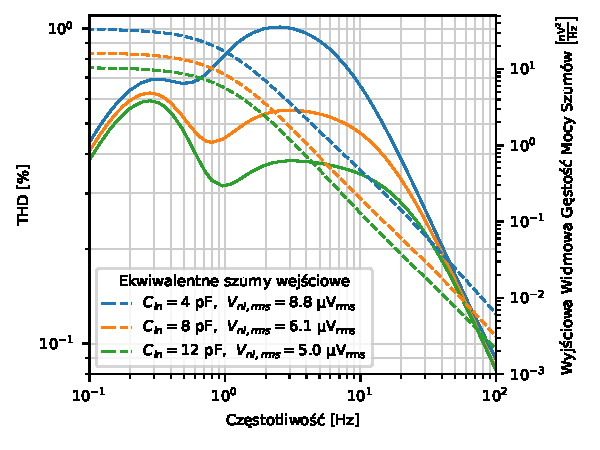
\includegraphics{scripts/tmp/thd_C_in.pdf} 
    \end{figure}

\end{frame}
